\documentclass[conference,a4paper]{IEEEtran}
\IEEEoverridecommandlockouts
% !TEX program = xelatex
% Unicode-safe, Times-compatible fonts for the original IEEEtran layout.
\usepackage{fontspec}
\setmainfont{Liberation Serif}[SmallCapsFont={Latin Modern Roman Caps}]
\setsansfont{Liberation Sans}
\setmonofont{Liberation Mono}[Scale=MatchLowercase]
\usepackage{seqsplit}
\usepackage{microtype}
\usepackage{amsmath,amssymb}
\usepackage{graphicx}
\usepackage{booktabs,multirow,array}
\usepackage{url}
\usepackage{balance}
\usepackage{cite}
\usepackage[hidelinks]{hyperref}
\newcommand{\map}{\mathrm{mAP}}
\newcommand{\AP}{\mathrm{AP}}
\newcommand{\D}{\mathrm{D}}
\newcommand{\M}{\mathrm{M}}
\title{How Much Does Road-Damage Detection Degrade Across Acquisition Domains?\\A Scene-Aware Bidirectional Evaluation on RDD2022}
\author{\IEEEauthorblockN{Lê Thành Luân\IEEEauthorrefmark{1}, Phạm Bá Anh Tuấn\IEEEauthorrefmark{2}}\IEEEauthorblockA{University of Science and Technology -- The University of Danang, Da Nang, Vietnam\\\IEEEauthorrefmark{1}102250416@hv.dut.udn.vn; \IEEEauthorrefmark{2}102250421@hv.dut.udn.vn}}
\begin{document}
\maketitle
\begin{abstract}
Road-damage detectors are often evaluated on imagery resembling their training data; however, deployment across camera platforms can reduce accuracy. This study aims to quantify the magnitude, asymmetry, and class dependence of cross-domain transfer between the China\_Drone and China\_MotorBike subsets of RDD2022. We use a scene-aware split and compare target-domain-trained and other-domain-trained detectors on identical held-out target images. The locked subset contains 4,378 images, including 658 test images, and four damage classes. COCO-pretrained YOLO11n, YOLOv8n, and YOLO26n are independently fine-tuned on each domain with three matched seeds and 150 epochs per run (18 runs). Mean fixed-target mAP@50:95 gaps range from 14.86 to 16.91 percentage points on Drone Test and from 41.24 to 42.94 points on MotorBike Test. For YOLO26n, the respective gaps are $16.91\pm0.80$ and $42.27\pm1.28$ points, where uncertainty is sample standard deviation over three seeds. All 18 seed-specific comparisons favor target-domain training. On MotorBike Test, D20 relative class-AP declines range from 96.14\% to 98.30\% against the target-trained baselines. YOLO26n improves mean in-domain mAP over YOLOv8n by 3.08 and 3.50 points on Drone and MotorBike, respectively, while substantial gaps persist. Our contribution is a reproducible bidirectional protocol and a three-variant replication of domain-associated asymmetry and class-specific vulnerability. Acquisition geometry, training size, and other collection differences remain jointly varying factors.
\end{abstract}
\begin{IEEEkeywords}
road damage detection, domain shift, RDD2022, YOLO11n, YOLOv8n, YOLO26n, scene-aware data splitting, reproducibility
\end{IEEEkeywords}
\section{Introduction}
Automated inspection of pavement distress is attractive because manual surveys are costly and difficult to repeat at scale. Early road-damage detection studies established vehicle-image benchmarks \cite{maeda2018road}, while RDD2022 provided a broader collection with four common damage categories \cite{arya2024rdd2022}. A detector fine-tuned on overhead images, however, may encounter very different object scales and road context when deployed with a camera mounted near road level. Whether such a detector retains its accuracy must be established empirically.

There is a common ambiguity in cross-domain evaluation. Comparing one model on two different test sets combines model transfer with differences in the intrinsic difficulty of those datasets. Instead, we compare a detector trained on the test domain against a detector trained on the other domain, \emph{using the same held-out target images}. We evaluate both transfer directions. This isolates test-set composition within a comparison, although it cannot isolate the causes of the training-domain difference.

We address four research questions: \textbf{RQ1}: How large and asymmetric are the fixed-target performance gaps? \textbf{RQ2}: Are gap directions and magnitudes consistent across random seeds and the three tested YOLO variants? \textbf{RQ3}: How does transfer vary among D00, D10, D20, and D40? \textbf{RQ4}: Does the addition of YOLO26n improve absolute accuracy while reducing or preserving domain-gap magnitude? \textbf{Our contributions are}: (1) a reproducible bidirectional evaluation with scene-aware partitions and fixed target test sets; (2) seed-resolved evidence of target asymmetry and class-specific vulnerability; and (3) replication across YOLO11n, YOLOv8n, and YOLO26n under matched explicit fine-tuning settings. The study provides a descriptive evaluation of source-domain choice rather than a new detector or an isolated causal estimate of viewpoint effects.

\section{Related Work}
\textbf{Consensus: domain shift degrades detection.} Multiple studies agree that learned predictors trained on one visual distribution suffer performance loss when deployed under different acquisition conditions. The domain-generalization literature cautions that success on source-like data may not carry to a shifted target distribution \cite{zhou2023survey}; benchmarks such as WILDS \cite{koh2021wilds} illustrate that preserving meaningful dataset boundaries is essential for valid performance claims. Road-damage detection follows this pattern: Maeda \emph{et al.} \cite{maeda2018road} introduced smartphone-image detection and classification, and Arya \emph{et al.} \cite{arya2024rdd2022} documented the multinational RDD2022 dataset's acquisition diversity, providing a setting in which camera-platform transfer can be examined.

\textbf{Trade-off: adaptation vs. controlled measurement.} One line of work develops architectures or adaptation strategies to improve cross-domain robustness. For example, YOLO-RD \cite{wang2025yolord} proposes detector enhancements for pavement distress. Such enhancement-oriented studies typically evaluate on a particular subset with architecture-specific tuning, making direct numerical comparison across papers difficult when dataset partitions, model sizes, label filtering, and validation protocols are not aligned. An alternative approach—adopted here—holds each detector's explicit fine-tuning settings fixed while varying the source acquisition domain, prioritizing a clear measurement of domain-associated performance differences.

\textbf{YOLO family evolution.} YOLOv8 \cite{ultralyticsyolov8}, YOLO11 \cite{jocher2024yolo11}, and YOLO26 \cite{ultralyticsyolo26} provide related compact detector variants with different pretrained checkpoints and model-specific implementations. Repeating the same fixed-target protocol across them tests whether the observed gap is confined to one variant. Matched explicit fine-tuning settings improve comparability, while architecture, pretraining, and implementation differences remain coupled.

\textbf{Gap: bidirectional asymmetry and class-level vulnerability.} Comparing one model on two different test sets conflates transfer behavior with intrinsic test-set difficulty. A fixed-target comparison is needed to quantify the advantage of target-domain training on each acquisition domain and to determine how that contrast varies across D00, D10, D20, and D40. The question addressed here is how large these two target-specific gaps are, whether their direction recurs across seeds and models, and which classes depart from the aggregate pattern.

\textbf{This paper.} We address the gap by measuring bidirectional fixed-target transfer between China\_Drone and China\_MotorBike subsets, using COCO-pretrained \cite{lin2014coco} YOLO11n \cite{jocher2024yolo11}, YOLOv8n \cite{ultralyticsyolov8}, and YOLO26n \cite{ultralyticsyolo26} to test whether the same qualitative pattern appears across three independently fine-tuned compact YOLO variants. We do not perform target-domain adaptation or use target images for model selection. Our contribution is an auditable evaluation protocol and a descriptive three-variant replication that measures asymmetry magnitude and class-specific vulnerability, not an architecture advance or a universal solution to domain shift.

\section{Data and Audit Protocol}
\subsection{Source and Label Ontology}
We use the China\_Drone (2,401 images) and China\_MotorBike (1,977 images) subsets from the publicly released RDD2022 dataset \cite{arya2024rdd2022}. The train/validation/test partitions below are the derived v4.1 partitions used in this study. Four shared object categories are retained: D00, longitudinal crack; D10, transverse crack; D20, alligator crack; and D40, pothole. The unit of detection evaluation is an annotated bounding box, not an independent physical defect or roadway site. The source domains differ in acquisition platform and potentially in location, surface condition, illumination, and label frequencies.

The primary measurement unit is average precision over annotated objects, while the reported seed-level variation reflects repeated training runs rather than independent roadway sites. The two image collections have unequal training sizes (1,680 versus 1,383), and ground-truth supports vary across classes and target domains. We consequently keep the full four-class mAP as the primary outcome and inspect class AP separately rather than post-hoc reweighting classes to raise the aggregate score.

\begin{table}[t]
\centering\caption{Locked v4.1 image counts by domain.}\label{tab:counts}
\begin{tabular}{lrrrr}\toprule
Domain & Train & Val & Test & Total\\\midrule
Drone & 1,680 & 360 & 361 & 2,401\\
MotorBike & 1,383 & 297 & 297 & 1,977\\\midrule
Total & 3,063 & 657 & 658 & 4,378\\\bottomrule
\end{tabular}
\end{table}

\begin{table}[t]
\centering\caption{Target-class bounding boxes in the locked test sets.}\label{tab:boxes}
\begin{tabular}{lrrrr}\toprule
Test & D00 & D10 & D20 & D40\\\midrule
Drone (361 images) & 214 & 189 & 44 & 17\\
MotorBike (297 images) & 403 & 165 & 96 & 35\\\bottomrule
\end{tabular}
\end{table}

\subsection{Scene-Aware Partitioning}
An earlier image/XML audit checked image–annotation correspondence, valid bounding boxes, class mapping, and candidate duplicate scenes. The review identified 735 high-priority visual-similarity pairs: 629 were marked same-scene, 93 different-scene, and 13 uncertain. AI-supported visual judgments were inspected and verified by the researcher; ambiguous cases retained the uncertainty label. Connected same-scene groups, uncertain pairs, and flagged medium/low-priority candidates were kept within a single train/validation/test partition under a conservative protection rule. This policy controls \emph{identified} cross-partition links; it does not prove that all possible duplicate scenes were found.

The locked split manifest SHA-256 is \texttt{\seqsplit{55c87dabc5da1ef500560648ec40717cde381dec0410b3abab83cbdfceed1322}}. Partition sizes are given in Table~\ref{tab:counts}. XML annotations outside the four target classes (including \texttt{Repair} and \texttt{Block crack}) were filtered, not remapped to D40. Excluded boxes are not automatic ignore regions in the primary evaluation. A sensitivity evaluation therefore uses image subsets without any excluded-class annotations: 273 Drone Test images and 271 MotorBike Test images. This subset comparison is descriptive because the test-image composition also changes.

\section{Experimental Design}
\subsection{Model Training}
Each architecture is initialized from its own fixed COCO-pretrained checkpoint: \texttt{yolo11n.pt}, \texttt{yolov8n.pt}, or \texttt{yolo26n.pt}. We train independently on Drone or MotorBike using seeds $\mathcal{S}=\{13,37,71\}$, yielding $3\times2\times3=18$ runs. No run is initialized from a previously fine-tuned run. All runs use 150 epochs, batch size eight, $640\times640$ input resolution, SGD with initial learning rate 0.01, momentum 0.937, weight decay 0.0005, and three warmup epochs. Mosaic and MixUp are off; translation, scale, and horizontal flip augmentation are applied uniformly. The highest-ranked checkpoint is selected by source-domain validation; test labels play no role in checkpoint selection. Training and evaluation were executed with Ultralytics 8.4.190 as recorded in the archives.

\subsection{Fixed-Target Evaluation and Statistics}
Each trained checkpoint is tested on both domains. Let $A_{m,s}(X\!\rightarrow\!Y)$ denote mAP@50:95 in percentage units of model $m$ trained on source $X$ with seed $s$ and evaluated on target $Y$. For a fixed target $Y$, the target-trained advantage is
\begin{equation}
G_{m,s}(Y)=A_{m,s}(Y\!\rightarrow\!Y)-A_{m,s}(X\!\rightarrow\!Y),\quad X\ne Y.
\label{eq:gap}
\end{equation}
Its three-seed mean and sample standard deviation are
\begin{align}
\bar{G}_m(Y)&=\frac{1}{3}\sum_{s\in\mathcal S}G_{m,s}(Y), \\[-2pt]
\sigma_m(Y)&=\sqrt{\frac{\sum_{s\in\mathcal S}(G_{m,s}(Y)-\bar G_m(Y))^2}{2}}.
\label{eq:std}
\end{align}
Gaps are reported in \emph{percentage points} (pp); a difference of 15~pp is not a 15\% relative decline. AP for each class and mAP@50 are also reported. With only three seeds, the sample standard deviations are descriptive and are not treated as confidence intervals or formal significance tests.

The matched-seed difference is used to standardize the summary design, not to imply that stochastic training paths in the two source collections are paired at the image level. All values below are based on the archived \texttt{best.pt} evaluations; an additional independent replay of per-image inference remains a verification step for future work.

\section{Results}
\subsection{RQ1: Bidirectional Fixed-Target Gaps}
Table~\ref{tab:matrix} contains the central result. All three models favor training on the evaluation domain, but the advantage is larger on MotorBike Test. For YOLO11n, the three-seed mean gap is $15.13\pm3.85$~pp on Drone Test versus $42.94\pm0.52$~pp on MotorBike Test. YOLOv8n shows corresponding gaps of $14.86\pm1.25$ and $41.24\pm1.04$~pp. YOLO26n adds corresponding gaps of $16.91\pm0.80$ and $42.27\pm1.28$~pp. This supports a strong, asymmetric \emph{association} between training acquisition domain and target performance; it is not a causal estimate of drone height or camera angle.

\begin{table*}[t]
\centering
\caption{Full-test mAP@50:95 (\%, mean $\pm$ sample SD over three seeds). The two rows for each architecture are tested on identical target images.}\label{tab:matrix}
\begin{tabular}{llrrr}\toprule
Architecture & Training domain & Drone Test & MotorBike Test & Seed count\\\midrule
\multirow{2}{*}{YOLO11n} & Drone & $22.39\pm1.82$ & $10.15\pm0.43$ & 3 \\
 & MotorBike & $7.25\pm3.64$ & $53.08\pm0.44$ & 3 \\
\multirow{2}{*}{YOLOv8n} & Drone & $21.41\pm1.71$ & $10.01\pm1.21$ & 3 \\
 & MotorBike & $6.55\pm2.59$ & $51.25\pm0.31$ & 3 \\
\multirow{2}{*}{YOLO26n} & Drone & $24.49\pm0.74$ & $12.48\pm0.13$ & 3 \\
 & MotorBike & $7.58\pm0.15$ & $54.75\pm1.24$ & 3 \\
\bottomrule
\end{tabular}
\end{table*}

\subsection{Convergence and Training Stability}
Figure~\ref{fig:training} presents the original representative training and validation trajectories for YOLO11n trained on Drone across three random seeds. Training loss declined steadily, while validation loss fluctuated before stabilizing. Maximum logged validation mAP@50:95 occurred at epochs 110, 92, and 111 for seeds 13, 37, and 71, respectively. Across the full experiment, all 18 runs completed 150 epochs with patience set to zero; the maximum logged validation-mAP epochs ranged from 63 to 133. The histories support completed, stable training under the stated budget. A pre-final-epoch validation peak does not establish global convergence or an optimal schedule, and maximum logged mAP alone does not independently verify the fitness rule used to save \texttt{best.pt}.

\begin{figure*}[t]
\centering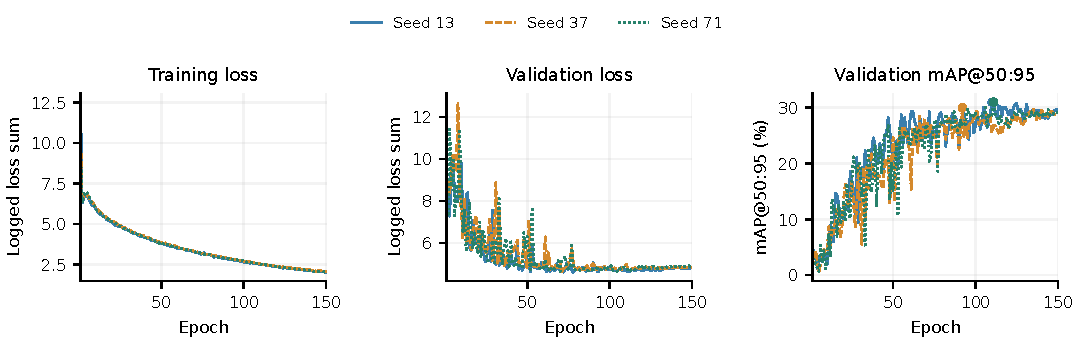
\includegraphics[width=\textwidth]{figures/training_curves.pdf}
\caption{Training and validation metrics for YOLO11n trained on Drone across seeds 13, 37, and 71. Left to right: summed logged training-loss components, summed logged validation-loss components, and validation mAP@50:95. Circles mark maximum logged mAP at epochs 110, 92, and 111; individual seed trajectories are shown without a shaded uncertainty band.}\label{fig:training}
\end{figure*}

\begin{figure}[t]
\centering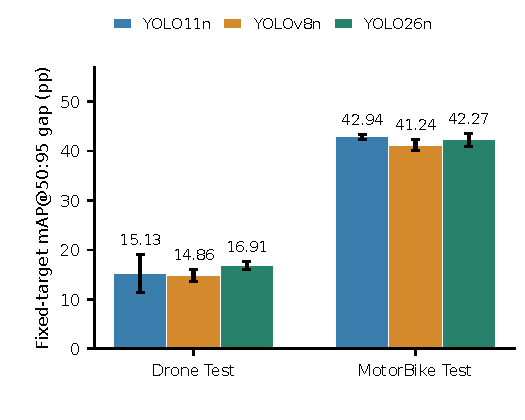
\includegraphics[width=\columnwidth]{figures/paired_gaps_comparison.pdf}
\caption{Mean same-target in-domain advantage in mAP@50:95 (pp). Error bars show sample SD over seeds, not confidence intervals.}\label{fig:gaps}
\end{figure}

\begin{table}[t]
\centering\caption{Full-test mAP@50 (\%, mean $\pm$ SD over three seeds), shown as a complementary metric.}\label{tab:map50}
\small\setlength{\tabcolsep}{4pt}
\begin{tabular}{llrr}\toprule
Model & Train & Drone & MotorBike\\\midrule
YOLO11n & Drone & $45.51\pm3.73$ & $23.44\pm2.34$ \\
YOLO11n & MotorBike & $20.81\pm11.78$ & $84.54\pm0.31$ \\
YOLOv8n & Drone & $44.17\pm2.77$ & $24.29\pm3.28$ \\
YOLOv8n & MotorBike & $18.02\pm6.99$ & $84.68\pm0.13$ \\
YOLO26n & Drone & $48.73\pm2.09$ & $27.47\pm0.44$ \\
YOLO26n & MotorBike & $18.11\pm0.61$ & $86.75\pm0.74$ \\
\bottomrule
\end{tabular}
\end{table}

\subsection{RQ2: Seed Stability and Architecture Replication}
For YOLO11n, paired gaps on Drone Test are 16.27, 10.84, and 18.29~pp for seeds 13, 37, and 71, respectively. On MotorBike Test they are 43.49, 42.47, and 42.85~pp. YOLOv8n reproduces the positive direction in all three seeds. Its Drone-target gaps are 15.03, 13.52, and 16.01~pp; its MotorBike-target gaps are 40.39, 42.40, and 40.93~pp. YOLO26n adds Drone-target gaps of 16.91, 16.10, and 17.71~pp and MotorBike-target gaps of 43.14, 42.87, and 40.80~pp. The gap \emph{direction} is replicated across all three variants and all 18 model--target--seed comparisons, while the seed-to-seed spread differs, especially on Drone Test. The three reused seed values and three variants from one model family support within-family replication; architectural changes remain coupled with pretraining and model-specific implementation differences.

\begin{table}[t]
\centering\caption{Paired fixed-target gap (pp), mean $\pm$ SD over seeds.}\label{tab:paired}
\begin{tabular}{lrr}\toprule
Model & Drone Test & MotorBike Test\\\midrule
YOLO11n & $15.13\pm3.85$ & $42.94\pm0.52$ \\
YOLOv8n & $14.86\pm1.25$ & $41.24\pm1.04$ \\
YOLO26n & $16.91\pm0.80$ & $42.27\pm1.28$ \\
\bottomrule
\end{tabular}
\end{table}

\begin{table}[t]
\centering\caption{Seed-specific fixed-target mAP@50:95 gaps (pp). All 18 values are positive.}\label{tab:seeds}
\begin{tabular}{llrrr}\toprule
Model & Test & Seed 13 & Seed 37 & Seed 71\\\midrule
YOLO11n & Drone & 16.27 & 10.84 & 18.29 \\
YOLO11n & MotorBike & 43.49 & 42.47 & 42.85 \\
YOLOv8n & Drone & 15.03 & 13.52 & 16.01 \\
YOLOv8n & MotorBike & 40.39 & 42.40 & 40.93 \\
YOLO26n & Drone & 16.91 & 16.10 & 17.71 \\
YOLO26n & MotorBike & 43.14 & 42.87 & 40.80 \\
\bottomrule
\end{tabular}
\end{table}

\subsection{RQ3: Class-Wise Heterogeneity}
Figure~\ref{fig:classes} compares the class-specific target-trained advantage. D00 and D10 show positive fixed-target differences on both targets. D20 shows a particularly large contrast on MotorBike Test, where all three variants reach substantially higher AP after training on MotorBike than after training on Drone. We retain D40 in all four-class primary metrics; we do not repair labels or change the split to improve observed AP. D40 is harder to interpret on Drone Test: only 17 annotated pothole boxes occur on nine images, many associated with one scene group, so AP changes can be dominated by a small number of detections.

Table~\ref{tab:classap} makes the class-specific variation explicit for \emph{all three} models. For MotorBike Test, D20 shows large target-trained advantages in each model (57.72, 53.21, and 56.45~pp for YOLO11n, YOLOv8n, and YOLO26n), whereas D40 on Drone Test shows negative mean fixed-target advantages ($-6.61$, $-9.74$, and $-1.95$~pp, respectively) with sparse support. This is an observational difference, not an architecture-level explanation of pothole recognition. The archived outputs do not provide an independent per-image false-positive/false-negative audit, so we do not attribute individual class failures to a particular visual mechanism.

\begin{figure}[t]
\centering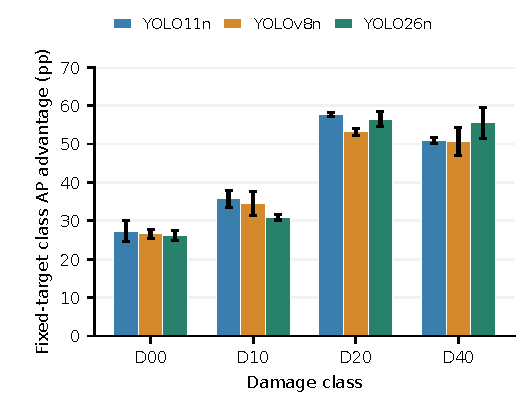
\includegraphics[width=\columnwidth]{figures/class_gap_motorbike.pdf}
\caption{Per-class fixed-target AP@50:95 advantage on MotorBike Test, averaged across three seeds. Positive bars favor MotorBike training.}\label{fig:classes}
\end{figure}

\begin{table*}[t]
\centering
\caption{Four-class AP@50:95 (\%, means over three seeds) on each fixed target. Rows with the same target contain identical held-out test images; higher class AP is not evidence that source differences are caused by camera viewpoint alone.}\label{tab:classap}
\begin{tabular}{lllrrrr}\toprule
Architecture & Training domain & Test domain & D00 & D10 & D20 & D40\\\midrule
YOLO11n & Drone & Drone & 32.45 & 36.48 & 17.42 & 3.20 \\
YOLO11n & MotorBike & Drone & 6.51 & 11.26 & 1.43 & 9.80 \\
YOLOv8n & Drone & Drone & 30.96 & 34.66 & 19.45 & 0.57 \\
YOLOv8n & MotorBike & Drone & 6.27 & 8.91 & 0.72 & 10.31 \\
YOLO26n & Drone & Drone & 33.37 & 39.57 & 22.94 & 2.06 \\
YOLO26n & MotorBike & Drone & 10.07 & 13.34 & 2.89 & 4.02 \\
YOLO11n & Drone & MotorBike & 20.98 & 17.35 & 1.00 & 1.26 \\
YOLO11n & MotorBike & MotorBike & 48.31 & 53.05 & 58.72 & 52.27 \\
YOLOv8n & Drone & MotorBike & 20.58 & 16.23 & 2.14 & 1.11 \\
YOLOv8n & MotorBike & MotorBike & 47.18 & 50.66 & 55.35 & 51.83 \\
YOLO26n & Drone & MotorBike & 24.27 & 22.75 & 1.54 & 1.38 \\
YOLO26n & MotorBike & MotorBike & 50.44 & 53.66 & 57.99 & 56.93 \\
\bottomrule
\end{tabular}
\end{table*}

\subsection{RQ4: Multi-Architecture Comparison}
Figure~\ref{fig:domain} compares all three variants on each fixed target. YOLO26n achieves the highest mean in-domain mAP@50:95: 24.49\% on Drone Test and 54.75\% on MotorBike Test. These exceed YOLOv8n by 3.08 and 3.50~pp, corresponding to relative gains of 14.38\% and 6.83\%. Its fixed-target gaps nevertheless remain 16.91 and 42.27~pp. Dividing each gap by the mean target-trained score on that same target gives relative declines of 69.04\% and 77.20\%. Thus, the additional model strengthens the original finding: higher in-domain mean accuracy does not eliminate the cross-domain deficit.

The effect is not a uniform ranking across classes or targets. YOLO11n retains higher in-domain D20 AP on MotorBike Test than YOLO26n (58.72\% versus 57.99\%). YOLO26n's MotorBike-target gap is slightly below YOLO11n's, while its Drone-target gap is larger. These three-seed comparisons do not establish the statistical significance of between-model differences.

\begin{figure*}[t]
\centering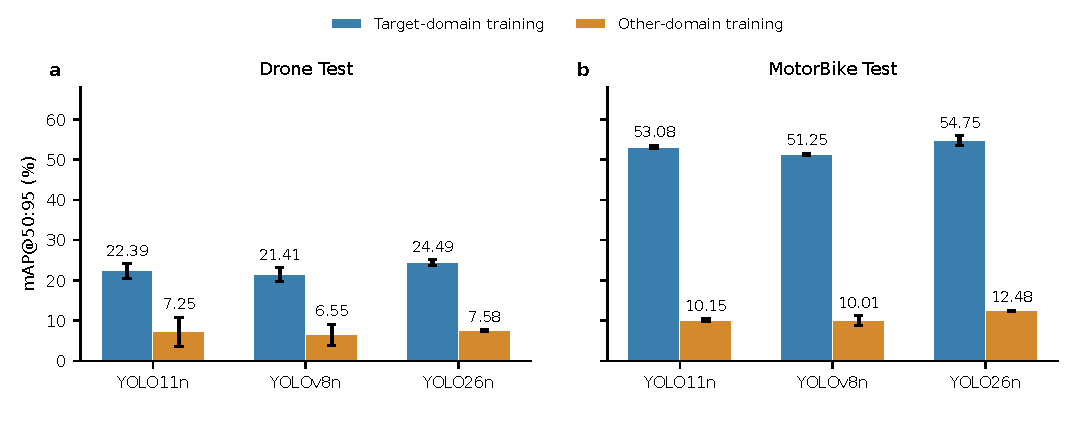
\includegraphics[width=\textwidth]{figures/domain_comparison.pdf}
\caption{Three-model comparison grouped by fixed target. Within each panel, target-domain-trained and other-domain-trained models are tested on identical held-out images. Bars show mean mAP@50:95 and error bars sample SD over seeds 13, 37, and 71. YOLO26n has higher in-domain mean scores while substantial target-specific gaps remain.}\label{fig:domain}
\end{figure*}

\subsection{Evaluation Sensitivity and Convergence}
All 18 training histories contain 150 recorded epochs, and checkpoint archives contain \texttt{best.pt} and \texttt{last.pt}. Validation peaks occur before the training budget ends, but the existence of a validation peak alone does not establish global convergence. Clean-only evaluations preserve the positive target-trained advantage in all 18 comparisons, with mean Drone/MotorBike gaps of 14.93/43.86~pp for YOLO11n, 15.25/41.87~pp for YOLOv8n, and 16.59/42.60~pp for YOLO26n; nevertheless, clean-only images differ from the full Test population, so the observed score change cannot be assigned only to excluded-label effects.

\section{Discussion}
The same-target design removes a major interpretive problem of subtracting scores from two different test sets. It does not equalize the sizes or composition of Drone and MotorBike training data (1,680 versus 1,383 images), nor their acquisition conditions. It is therefore more precise to describe the result as a \emph{domain-associated source-training gap} than an experimentally isolated viewpoint effect. A substantial positive gap appears across all three compact YOLO variants and all seed-specific comparisons, especially when MotorBike is the target; this is the empirical finding supported by the archive.

\textbf{Why does performance degrade?} Three factors provide hypotheses for interpreting the observed domain gap. First, \textbf{scale mismatch}: overhead and near-ground imagery can present defects at different pixel scales and perspectives, potentially changing the visual information available to a detector. Object-scale distributions and paired views were not measured here, so a scale mechanism remains to be tested. Second, \textbf{context distribution shift}: different roadway framing and surrounding backgrounds may alter source-domain cues. The fixed-target contrast shows that source choice matters but does not distinguish context from illumination, road-surface differences, or annotation density. Third, \textbf{class-specific fragility}: on MotorBike Test, D20 AP falls from 58.72\% to 1.00\% for YOLO11n, from 55.35\% to 2.14\% for YOLOv8n, and from 57.99\% to 1.54\% for YOLO26n when target-domain training is replaced by Drone training. Relative to the target-trained class means, these declines are 98.30\%, 96.14\%, and 97.34\%; D00 declines on the same target are smaller at 56.57\%, 56.37\%, and 51.88\%. Fine-texture and scale sensitivity are plausible explanations for this class contrast, requiring controlled or per-image analysis to establish their roles.

\textbf{Comparison with prior work.} Our findings support the motivation for distribution-aware evaluation in domain-generalization research and WILDS \cite{zhou2023survey,koh2021wilds}, while focusing on two road-acquisition domains and their class-specific contrasts. The fixed-target protocol complements detector-enhancement work such as YOLO-RD \cite{wang2025yolord}; we do not numerically rank studies with incompatible partitions and label policies. COCO \cite{lin2014coco} supplies the pretraining context rather than evidence of adaptation on these road datasets. The MotorBike-target advantage exceeds the Drone-target advantage by 27.80, 26.38, and 25.36~pp for YOLO11n, YOLOv8n, and YOLO26n, respectively. This quantifies the difference between two target-specific gaps without establishing that either acquisition platform intrinsically produces more transferable features.

\subsection{Limitations}
Several design choices bound the interpretation. Training sizes differ (1,680 versus 1,383 images), and acquisition domain can also vary with location, roadway condition, illumination, and annotation density. No balancing or ablation study separates these factors. Three seed values and three compact variants from one YOLO family support replication on the fixed datasets, not precise population-level inference or architecture-independent generalization. Both domains are China subsets, so transfer to other countries and devices remains unmeasured. D40 has sparse Drone support, and filtered classes outside D00--D40 are not ignore regions. These constraints motivate targeted controls rather than treating the observed gaps as isolated viewpoint effects.

\subsection{Threats to Validity}
The scene-review and conservative grouping address identified similarity candidates but cannot guarantee that all latent scene overlap was found. Some MotorBike images were encountered during exploratory analysis before split finalization, limiting an entirely untouched-holdout claim. Clean-only evaluation retains the gap direction but changes the image population. The present analysis checks and recomputes archived metric summaries; it does not independently rerun inference from each checkpoint on every original test image or replay the original image/XML audit. Seed SDs are descriptive and do not replace scene-level uncertainty estimates.

To strengthen the analysis beyond the current descriptive experiment, a source-size-matched training control and a scene-stratified bootstrap based on saved per-image predictions would be useful. A paired-view data collection on the same road sections would be needed to isolate acquisition geometry. Evaluating Czech or India from RDD2022, or an independent dataset, requires a separate label-ontology audit and should not be folded into the present 18-run result.

The study establishes a seed-resolved, descriptive replication of domain-associated gaps on the locked partition. The next controls should test the source-size, scene-composition, and acquisition-geometry explanations identified above.

\section{Conclusion}
On the scene-reviewed RDD2022 v4.1 Drone/MotorBike split, 18 fine-tuning runs across YOLO11n, YOLOv8n, and YOLO26n show consistent in-domain advantages under fixed-target evaluation. Mean gaps range from 14.86 to 16.91~pp on Drone Test and from 41.24 to 42.94~pp on MotorBike Test, with distinct class-level behavior. \textbf{Key quantitative findings:} (1) all 18 full-test seed comparisons and their clean-only counterparts favor target-domain training; (2) MotorBike-target D20 relative AP declines range from 96.14\% to 98.30\% against the target-trained baselines, while sparse Drone-target D40 shows negative mean class gaps; and (3) MotorBike-target advantages exceed Drone-target advantages by 25.36--27.80~pp across the three variants. YOLO26n raises in-domain mean accuracy while preserving the substantial cross-domain gap. The contribution is a seed-resolved, three-variant comparison of source-domain choice on fixed target test sets.

\textbf{Practical implications:} Practitioners deploying road-damage detectors across camera platforms should budget for substantial mAP degradation, validate performance on the intended target platform, and prioritize retraining or domain adaptation when acquisition geometry changes. Class-level validation is important because aggregate mAP can hide large D20 losses and sparse-class reversals. \textbf{Future work} should validate per-image predictions independently, quantify scene-level uncertainty, test additional acquisition domains (India, Czech, Japan subsets) under an unchanged audit protocol, and explore multi-domain training strategies to improve cross-platform robustness.

\section*{Data Availability and Declarations}
The source RDD2022 dataset is cited in \cite{arya2024rdd2022}. The derived experiment uses locked manifest SHA-256 \texttt{\seqsplit{55c87dabc5da1ef500560648ec40717cde381dec0410b3abab83cbdfceed1322}}. Accompanying CSV files contain every archived full/clean-only metric row, training-run metadata, and summary tables; model checkpoints and original imagery are not redistributed with the manuscript source. The recorded scene review was AI-assisted and checked by the researcher; manuscript editing and figure preparation also used AI assistance. Author contributions, conflicts of interest, funding, and any venue-required AI-use declaration must be validated by the authors before submission.

\balance
\bibliographystyle{ieeetr}
\bibliography{references}
\end{document}
